\documentclass[11pt]{article}

\usepackage{pablo-devoir}
\usepackage[a5paper,margin=1cm]{geometry}
\usepackage{subcaption}

\pagestyle{empty}

\title{{\normalsize Fonctions Histogramme} Corrigé}
\date{07/01/15}
\classe{2\up{des}14}
\dsnum{DM 3}

\begin{document}

\maketitle

\begin{figure}[h]
  \label{figure:courbes}
  \centering
  \begin{subfigure}[t]{0.5\textwidth}
    \centering
    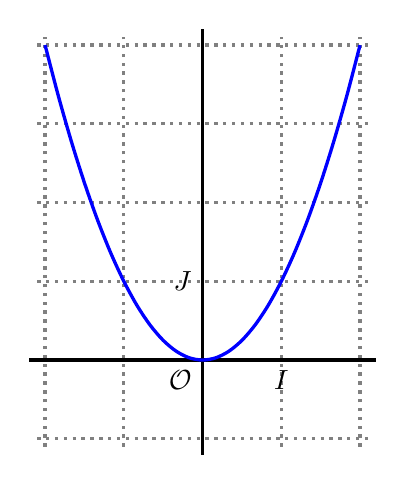
\begin{tikzpicture}[domain=-2:2, very thick]
      \draw[dotted,color=gray] (-2.1,-1.1) grid (2.1,4.1);
      \draw[] (-2.2,0) -- (2.2,0);
      \draw[] (0,-1.2) -- (0,4.2);

      \draw (0,0) node[below left]{$\mathcal{O}$};
      \draw (1,0) node[below]{$I$};
      \draw (0,1) node[left]{$J$};

      \draw[domain=-2:2,smooth,blue] plot ({\x},{\x*\x});
    \end{tikzpicture}
    \caption{Exercice \ref{exo:carree}}
  \end{subfigure}%
  ~
  \begin{subfigure}[t]{0.5\textwidth}
    \centering
    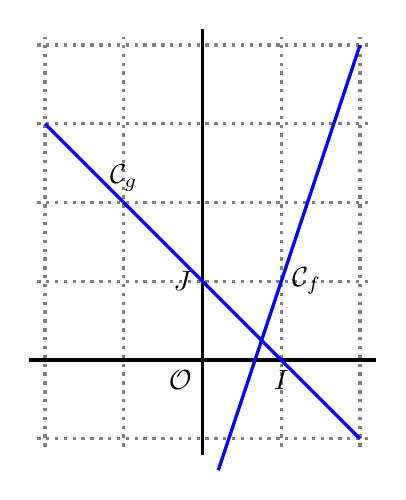
\begin{tikzpicture}[domain=-2:2,very thick]
      \draw[dotted,color=gray] (-2.1,-1.1) grid (2.1,4.1);
      \draw[] (-2.2,0) -- (2.2,0);
      \draw[] (0,-1.2) -- (0,4.2);

      \draw (0,0) node[below left]{$\mathcal{O}$};
      \draw (1,0) node[below]{$I$};
      \draw (0,1) node[left]{$J$};

      \draw[domain=.2:2,smooth,blue] plot ({\x},{3*\x-2});
      \draw(1,1) node[right]{$\mathcal{C}_f$};

      \draw[domain=-2:2,smooth,blue] plot ({\x},{-\x+1});
      \draw(-1,2) node[above]{$\mathcal{C}_g$};
    \end{tikzpicture}
    \caption{Exercice \ref{exo:droites}}
  \end{subfigure}
  \caption{Représentations graphiques}
\end{figure}

\begin{exercice}[Variation de la fonction carrée]\label{exo:carree}
  \emph{Le but de l'exercice est d'étudier les variations de la fonction $f:x\mapsto x^2$, définie sur $\mathbb{R}$ (appellée \emph{fonction carrée}).}

  \begin{enumerate}
    \item \emph{Rappeler la définition de \emph{fonction croissante} et \emph{fonction décroissante}.}
      \label{question:definitions}
      \begin{itemize}
        \item Une fonction $f$ définie sur un intervalle $I$ est dite croissante si pour tout $a$ et $b$ de $I$, si $a<b$, alors $f(a)\leq f(b)$.
        \item Elle est dite décroissante si pour tout $a$ et $b$ de $I$, si $a<b$, alors $f(a)\geq f(b)$.
      \end{itemize}
    \item 
      \begin{enumerate}
        \item \emph{Dans un repère orthonormé, tracer la courbe représentative de $f$, pour des abscisses allant de $-2$ à 2, et des ordonnées de $-4$ à 4.}
          Voir le graphique page \pageref{figure:courbes}.
        \item \emph{Par lecture graphique, conjecturer les variations de $f$.}

          \label{question:variations-carree}
    \begin{tikzpicture}
      \tkzTabInit[lgt=2,espcl=2]
      {$x$ /1,
      $x^2$ /2}
      {$-\infty$,$0$,$+\infty$}%
      \tkzTabVar{+/, -/0, +/}
    \end{tikzpicture}
      \end{enumerate}
    \item \emph{Soient $a$ et $b$ deux nombres positifs, tels que $a<b$.}
      \begin{enumerate}
        \item \emph{Quel est le signe de $a+b$ ? Quel est le signe de $a-b$ ?}
          Les nombres $a$ et $b$ étant positifs, $a+b$ est positif. Puisque $a<b$, alors $a-b<0$.
        \item \emph{En déduire le signe de $\left( a+b \right)\left( a-b \right)$.}
          D'après la question précédente, le produit $\left( a+b \right)\left( a-b \right)$ est le produit d'un nombre positif et d'un nombre négatif : il est négatif.
        \item
            \emph{En déduire que $a^2<b^2$.}
          \begin{align*}
            \left( a+b \right)\left( a-b \right) &< 0 \\
            a^2-b^2 &<0 \\
            a^2 &< b^2
          \end{align*}
        \item \emph{En déduire le sens de variations de $f$ sur $\left[ 0; +\infty \right[$.}
            Nous avons montré que, $a$ et $b$ étant des nombres positifs, si $a<b$, alors $f(a)<f(b)$ (puisque $f(a)=a^2$ et $f(b)=b^2$). C'est la définition même d'une fonction croissante : $f$ est croissante sur les nombres réels positifs (sur $\left[ 0; +\infty \right[$).
        \end{enumerate}
    \item \emph{Refaire le même raisonnement avec $a$ et $b$ deux nombres négatifs, et en déduire le sens de variations de $f$ sur $\left] -\infty;0 \right]$.}
      Soient $a$ et $b$ deux nombres négatifs tels que $a<b$.

      Considérons le produit $\left( a+b \right)\left( a-b \right)$ : chacun des deux membres $a+b$ et $a-b$ est négatif, donc le produit est positif. Donc :
      \begin{multicols}{2}
      \begin{align*}
        \left( a+b \right)\left( a-b \right) &>0 \\
        a^2-b^2 &> 0 \\
        a^2 &> b^2 \\
        f(a) &> f(b)
      \end{align*}

      Nous avons montré que si $a<b$, alors $f(a)>f(b)$. Donc la fonction carrée est positive sur les nombres négatifs.
    \end{multicols}
    \item \emph{Conclure en dressant le tableau de variations de $f$ sur $\mathbb{R}$.}
      Le tableau de variations de $f$ est bien celui conjecturé en question \ref{question:variations-carree}.

  \end{enumerate}

\end{exercice}

\begin{exercice}[Variations d'une fonction affine]\label{exo:droites}
  \emph{Le but de l'exercice est d'étudier les variations des fonctions $f:x\mapsto 3x-2$ et $g:x\mapsto -x+1$.}
  \begin{enumerate}
    \item \emph{Rappeler la définition de \emph{fonction croissante} et \emph{fonction décroissante}.}
      Voir question \ref{question:definitions} de l'exercice précédent.
    \item \emph{Tracer dans un repère orthonormé les courbes de $f$ et $g$, et donner leurs variations par lecture graphique.}
        Pour le graphique, voir page \pageref{figure:courbes}. Voici les tableaux de variations.

      \begin{multicols}{2}
        \begin{center}
        \begin{tikzpicture}
          \tkzTabInit[lgt=1,espcl=2]
          {$x$ /1,
          $f$ /2}
          {$-\infty$,$+\infty$}%
          \tkzTabVar{-/, +/}
        \end{tikzpicture}
      \end{center}

      \begin{center}
        \begin{tikzpicture}
          \tkzTabInit[lgt=1,espcl=2]
          {$x$ /1,
          $g$ /2}
          {$-\infty$,$+\infty$}%
          \tkzTabVar{+/, -/}
        \end{tikzpicture}
      \end{center}
      \end{multicols}
    \item \emph{Étude de $f$. Soient $a$ et $b$ deux nombres tels que $a<b$.}
      \begin{enumerate}
        \item \emph{Compléter le raisonnement suivant avec les signes $<$ et $>$.}
          \begin{align*}
            a &< b\\
            3a & < 3b\\
            3a-2 &< 3b-2\\
            f(a) &< f(b)
          \end{align*}
        \item \emph{En déduire le sens de variations de $f$.}
          Nous avons montré que si $a<b$, alors $f(a)<f(b)$: c'est la définition même d'une fonction croissante. La fonction $f$ est donc croissante sur $\mathbb{R}$.
      \end{enumerate}
    \item \emph{\emph{Étude de $g$.} Soient $a$ et $b$ deux nombres tels que $a<b$.}
      \begin{enumerate}
        \item \emph{Compléter le raisonnement suivant avec les signes $<$ et $>$, et en justifiant le passage à la deuxième ligne.}
          \begin{align*}
            a &< b\\
            -a & > -b \text{\hspace{1cm}car on a multiplié par un nombre négatif}\\
            -a+1 &> -b+1\\
            g(a) &> g(b)
          \end{align*}
        \item \emph{En déduire le sens de variations de $g$.}
          Nous avons montré que si $a<b$, alors $g(a)>g(b)$. C'est la définition même de la décroissance d'une fonction. Donc la fonction $g$ est décroissante sur l'ensemble des réels $\mathbb{R}$.
      \end{enumerate}
  \end{enumerate}
\end{exercice}

\begin{exercice}[Histogramme à classes irrégulières]
  \emph{Alain, intéressé par la météorologie, mesure les précipitations chez lui
    toutes les semaines. Il part quinze jours en vacances entre les 36\up{e} et 50\up{e} jour, et n'a donc pu faire qu'un seul relevé pour l'ensemble de ces deux semaines.}
  
  ~

  \hspace{-2.5em}\begin{tabular}{p{2cm}||c|c|c|c|c|c|c}
    Jours &
    $\left[ 1; 8 \right[$ &
    $\left[ 8; 15 \right[$ &
    $\left[ 15; 22 \right[$ &
    $\left[ 22; 29 \right[$ &
    $\left[ 29; 36 \right[$ &
    $\left[ 36; 50 \right[$ &
    $\left[ 50; 57 \right[$ \\
    \hline
    Précipita\-tions (mm) & 15 & 14 & 14 & 16 & 17 & 31 & 16 \\
  \end{tabular}

  \emph{Le tableau se lit de la manière suivante : Sur l'ensemble des sept premiers jours, il est tombé 15~mm d'eau.}

  \begin{enumerate}
    \item \emph{Étude des jours 36 à 50.}
      \begin{enumerate}
        \item \emph{Calculer la hauteur moyenne d'eau tombée par jour du 29\up{e} au 36\up{e} jour, puis la hauteur moyenne d'eau tombée par jour du 36\up{e} au 50\up{e} jour.}
          Il a plu 17~mm du 29\up{e} au 36\up{e} jour, soit 17~mm en sept jours, soit $\frac{17}{7}\approx2,4$ milimètres par jour.

          Du 36\up{e} au 50\up{e} jour, il a plu 31~mm, soit $\frac{31}{14}\approx2,2$ milimètres par jour.
        \item \emph{Est-il tombé beaucoup plus d'eau de 36\up{e} au 50\up{e} jour que pendant le reste de l'étude ?}
          Il n'est pas tombé plus d'eau entre le 36\up{e} et le 50\up{e} jour que le reste de l'étude.
      \end{enumerate}
  \end{enumerate}

  \emph{Afin de visualiser les précipitations, Alain trace l'histogramme suivant.}

  \begin{center}
    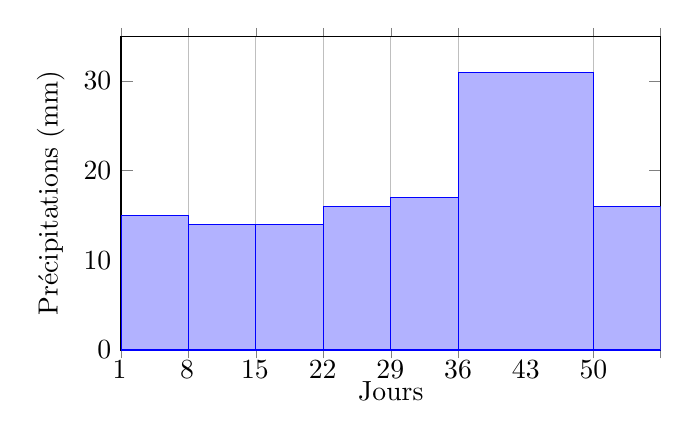
\begin{tikzpicture}
      \begin{axis}[
          yscale=0.7,
          ymin=0,
          ymax=35,
          xmin=1,
          xmax=57,
          xlabel={Jours},
          ylabel={Précipitations (mm)},
          ybar interval,
          xticklabel={~},
        ]
        \addplot coordinates {
          (1, 15)
          (8, 14)
          (15, 14)
          (22, 16)
          (29, 17)
          (36, 31)
          (50, 16)
          (57, 0)
        };
      \end{axis}
      \foreach \x in {1, 8, ..., 50} {
        \draw[thick] ({.12286*\x-0.1429}, 0) node[below]{\x};
    }
    \end{tikzpicture}
  \end{center}
  \begin{enumerate}
      \setcounter{enumi}{1}
    \item \emph{Selon son histogramme, pendant quels jours ont eu lieu les plus fortes précipitations ? Cela reflète-t-il la réalité (comparer cela avec le résultat de la question précédente) ?}
      La barre entre les 36\up{e} et 50\up{e} jours est beaucoup plus haute que les autres, donc on a l'impression qu'il a davantage plu durant cette période. Mais nous avons montré dans la question précédente que ce n'était pas le cas. Donc l'histogramme ne reflète pas la réalité.
  \end{enumerate}
  \begin{em}
  L'erreur d'Alain est qu'il a fait \emph{les hauteurs} des barres proportionnelles à
  la valeur des caractères, alors que \emph{les aires} des barres auraient dû être
  proportionnelles à la valeur des caractères.

  Le but de cet exercice est de tracer un histogramme correct.
\end{em}

  \begin{enumerate}
      \setcounter{enumi}{2}
    \item \begin{em}
        Dans cette question nous allons compléter le tableau de
      proportionnalité suivant, où les trois dernières lignes correspondent aux
      barres de l'histogramme que nous tracerons ensuite.
      \end{em}

      \hspace{-3.5em}\begin{tabular}{p{2cm}||c|c|c|c|c|c|c}
    Jours &
    $\left[ 1; 8 \right[$ &
    $\left[ 8; 15 \right[$ &
    $\left[ 15; 22 \right[$ &
    $\left[ 22; 29 \right[$ &
    $\left[ 29; 36 \right[$ &
    $\left[ 36; 50 \right[$ &
    $\left[ 50; 57 \right[$ \\
          \hline
          \hline
          Précipita\-tions (mm) & 15 & 14 & 14 & 16 & 17 & 31 & 16 \\
          \hline
          \hline
          Aire &  30 & 28 & 28 & 32 & 34 & 62 & 32 \\
          \hline
          Largeur & 7 & 7& 7& 7& 7& 14& 7\\
          \hline
          Hauteur & 4,3 & 4 & 4 & 4,6 & 4,9 & 4,4 & 4,6
        \end{tabular}

      \begin{enumerate}[(a)]
        \item \emph{Remplir la ligne « Aire », de sorte que l'aire soit proportionnelle aux précipitations.}
          Voir le tableau.
        \item \emph{Remplir la ligne « Hauteur », de sorte que dans chaque colonne, le produit de la hauteur par la largeur soit égale à l'aire.}
          Voir le tableau.
      \end{enumerate}
    \item \emph{Tracer l'histogramme en utilisant les largeurs et hauteurs des barres calculées dans le tableau.}
  \begin{center}
    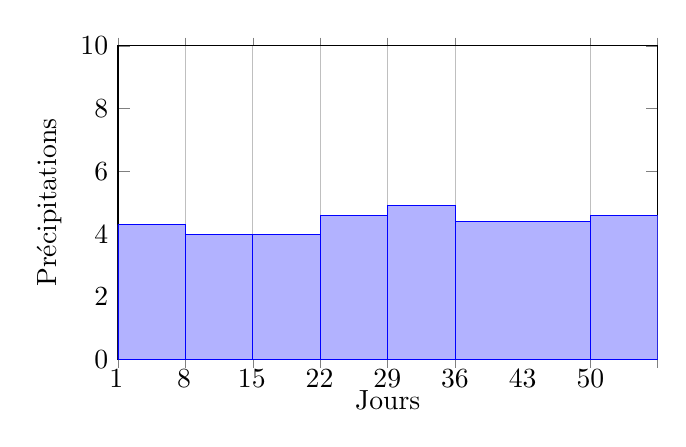
\begin{tikzpicture}
      \begin{axis}[
          yscale=0.7,
          ymin=0,
          ymax=10,
          xmin=1,
          xmax=57,
          xlabel={Jours},
          ylabel={Précipitations},
          ybar interval,
          xticklabel={~},
        ]
        \addplot coordinates {
          (1, 4.3)
          (8, 4)
          (15, 4)
          (22, 4.6)
          (29, 4.9)
          (36, 4.4)
          (50, 4.6)
          (57, 0)
        };
      \end{axis}
      \foreach \x in {1, 8, ..., 50} {
        \draw[thick] ({.12286*\x-0.1429}, 0) node[below]{\x};
    }
    \end{tikzpicture}
  \end{center}

    \item \emph{Application : Dans une étude de 2011 commandée par la \textsc{Hadopi} figurent les chiffres suivants, qui décrivent la somme moyenne dépensée chaque mois en produits et services culturels par les internautes ayant l'habitude de télécharger de manière illégale.}

      \begin{center}
        \begin{tabular}{p{4cm}|c|c|c|c}
          Somme dépensée (\euro)
          & $\left] 0;20 \right[$
          & $\left[ 20;31 \right[$
          & $\left[ 31;100 \right[$
          & $\left[ 100;500 \right[$
          \\
          \hline
          Effectif
          & 342
          & 369
          & 250
          & 118
          \\
          \hline
          Largeur & 20 & 10 & 70 & 400 \\\hline
          Aire & 342 & 369 & 250 & 118 \\\hline
          Hauteur & 17,1 & 36,9 & 3,57 & 0,295 \\\hline
        \end{tabular}
      \end{center}
      \emph{Représenter ces données dans un histogramme.}

      Nous remplissons le tableau avec la même méthode que précédemment :
      \begin{itemize}
        \item Nous ajoutons une ligne \emph{Largeur}, représentant la largeur de chaque barre, et correspondant à l'amplitude de l'intervalle de la somme dépensée.
        \item Nous ajoutons une ligne contenant l'aire de chacune des barres. Nous choisissons ici comme aire l'effectif (ainsi, de manière triviale, l'aire est proportionnelle à l'effectif).
        \item Nous calculons la hauteur comme la division de l'aire par la largeur.
      \end{itemize}
      Cela donne l'effectif suivant :

  \begin{center}
    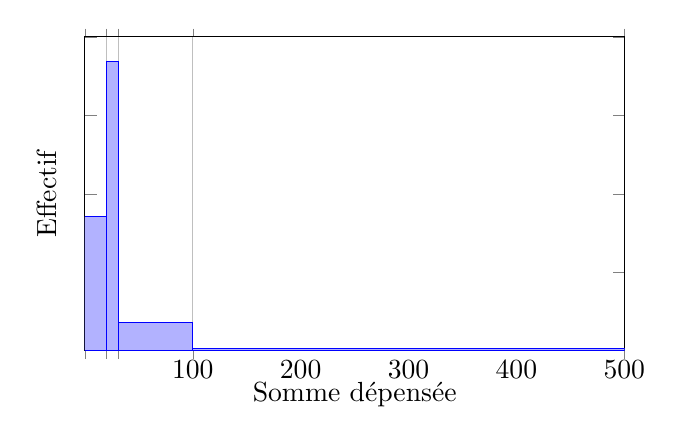
\begin{tikzpicture}
      \begin{axis}[
          yscale=0.7,
          ymin=0,
          ymax=40,
          xmin=0,
          xmax=500,
          xlabel={Somme dépensée},
          ylabel={Effectif},
          ybar interval,
          xticklabel={~},
          yticklabel={~},
        ]
        \addplot coordinates {
          (0, 17.1)
          (20, 36.9)
          (31, 3.57)
          (100, 0.295)
          (500, 0)
        };
      \end{axis}
      \foreach \x in {1, 2, ..., 5} {
        \draw[thick] ({1.37*\x}, 0) node[below]{\x00};
    }
    \end{tikzpicture}
  \end{center}

  \end{enumerate}
\end{exercice}

\end{document}
